% Apresentação: IA Generativa como propulsora das Redes de Cooperação Extensionistas
% Autor: Ney Lemke

\documentclass[aspectratio=169,12pt]{beamer}

% Pacotes necessários
\usepackage[utf8]{inputenc}
\usepackage[brazilian]{babel}
\usepackage{amsmath,amsfonts,amssymb}
\usepackage{graphicx}
\usepackage{xcolor}
\usepackage{tikz}
\usepackage{fontawesome5}
\usepackage{hyperref}

% Configuração do tema dark
\usetheme{Madrid}
\usecolortheme{beaver}

% Cores personalizadas para dark mode
\definecolor{darkbg}{RGB}{26,26,26}
\definecolor{darkfg}{RGB}{229,229,229}
\definecolor{accent}{RGB}{102,126,234}
\definecolor{secondary}{RGB}{118,75,162}
\definecolor{success}{RGB}{34,197,94}
\definecolor{warning}{RGB}{251,191,36}
\definecolor{danger}{RGB}{239,68,68}

% Configuração das cores do tema
\setbeamercolor{background canvas}{bg=darkbg}
\setbeamercolor{normal text}{fg=darkfg}
\setbeamercolor{structure}{fg=accent}
\setbeamercolor{title page}{fg=darkfg}
\setbeamercolor{frametitle}{fg=darkfg,bg=accent}
\setbeamercolor{block title}{fg=white,bg=accent}
\setbeamercolor{block body}{fg=darkfg,bg=darkbg!80}
\setbeamercolor{block title alerted}{fg=black,bg=danger}
\setbeamercolor{block title example}{fg=black,bg=success}
\setbeamercolor{block body alerted}{fg=black,bg=danger!20}
\setbeamercolor{block body example}{fg=black,bg=success!20}
\setbeamercolor{item}{fg=accent}
\setbeamercolor{navigation symbols}{bg=darkbg,fg=darkfg}

% Remover símbolos de navegação
\setbeamertemplate{navigation symbols}{}

% Customizar footline
\setbeamertemplate{footline}[frame number]

% Configurações de hyperlink
\hypersetup{
    colorlinks=true,
    linkcolor=accent,
    urlcolor=accent,
    citecolor=accent
}

% Informações da apresentação
\title[IA \& Extensão]{IA Generativa como Propulsora das Redes de Cooperação Extensionistas}
\subtitle{Agência e Impacto Social na Universidade do Futuro}
\author{Ney Lemke}

\institute{Unesp}
\date{\today}

\begin{document}

% SLIDE DE ABERTURA
\begin{frame}
    \titlepage
    \begin{center}
        \textcolor{accent}{\faRobot\, \faHandsHelping\, \faGraduationCap}
    \end{center}
\end{frame}

% ============================================================================
% AGENDA - DIVIDIDA PARA EVITAR OVERFLOW
% ============================================================================

\begin{frame}[shrink]{Agenda: Parte 1 - Fundamentos e Abundância}
    \begin{columns}[T]
        \begin{column}{0.48\textwidth}
            \begin{block}{\faListOl\, Introdução}
                \begin{enumerate}
                    \item<1-> \textbf{Introdução à IA Generativa}
                    \begin{itemize}
                        \item O que é a IA que "cria"?
                        \item Como funcionam os LLMs
                    \end{itemize}

                    \item<2-> \textbf{Software 3.0}
                    \begin{itemize}
                        \item A evolução para a linguagem natural
                        \item Democratização da programação
                    \end{itemize}
                \end{enumerate}
            \end{block}
        \end{column}

        \begin{column}{0.48\textwidth}
            \begin{block}{\faListOl\, O Reflexo}
                \begin{enumerate}
                    \setcounter{enumi}{2}
                    \item<3-> \textbf{A Abundância da Inteligência}
                    \begin{itemize}
                        \item O fim do monopólio do conhecimento na universidade
                        \item Inteligência como \textit{commodity}
                    \end{itemize}
                \end{enumerate}
            \end{block}
            \vspace{0.5cm}
            \begin{exampleblock}{\faLightbulb\, O Paradigma Inicial}
                \centering
                A IA redefiniu o que significa ser "capaz" no cenário acadêmico atual.
            \end{exampleblock}
        \end{column}
    \end{columns}
\end{frame}

\begin{frame}[shrink]{Agenda: Parte 2 - Ação e Governança}
    \begin{columns}[T]
        \begin{column}{0.48\textwidth}
            \begin{block}{\faListOl\, A Nova Fronteira Humana}
                \begin{enumerate}
                    \setcounter{enumi}{3}
                    \item<1-> \textbf{O Que é "Agência"?}
                    \begin{itemize}
                        \item Agir frente à incerteza
                        \item O risco da pura "veneração da inteligência"
                    \end{itemize}
                    
                    \item<2-> \textbf{Novo Modelo Educacional}
                    \begin{itemize}
                        \item Aprender perguntando
                        \item Tolerância à Falha Produtiva
                    \end{itemize}
                \end{enumerate}
            \end{block}
        \end{column}

        \begin{column}{0.48\textwidth}
            \begin{block}{\faListOl\, Instituição em Aplicação}
                \begin{enumerate}
                    \setcounter{enumi}{5}
                    \item<3-> \textbf{Ações e Governança da Unesp}
                    \begin{itemize}
                        \item A Resolução Unesp 13/2025
                        \item Uso ético e ampliação humana
                    \end{itemize}
                    
                    \item<4-> \textbf{Redes de Cooperação Extensionistas}
                    \begin{itemize}
                        \item Agência testada no mundo real
                        \item IA como suporte estrutural
                    \end{itemize}
                \end{enumerate}
            \end{block}
            \vspace{0.5cm}
            \begin{exampleblock}{\faLightbulb\, O Paradigma}
                \centering
                A adaptação é a chave para a sobrevivência acadêmica.
            \end{exampleblock}
        \end{column}
    \end{columns}
\end{frame}

% ============================================================================
% SEÇÃO 1: INTRODUÇÃO À IA GENERATIVA
% ============================================================================

\section{Introdução à IA Generativa}

%\begin{frame}{Inteligência Artificial no Imaginário Popular}
    %\begin{columns}
        %\begin{column}{0.4\textwidth}
            %\begin{block}{Expectativa vs Realidade}
                %A cultura pop moldou nossa visão sobre a IA durante décadas:
                %\begin{itemize}
                    %\item \textbf{O Lógico e Frio:} HAL 9000 (2001)
                    %\item \textbf{O Humano Sintético:} Replicantes (Blade Runner)
                    %\item \textbf{O Assistente Perfeito:} J.A.R.V.I.S (Homem de Ferro)
                    %\item \textbf{O Autônomo Empático:} Wall-E
                %\end{itemize}
            %\end{block}
        %\end{column}
        %\begin{column}{0.6\textwidth}
            %\begin{center}
                %% ATENÇÃO: Salve a imagem enviada no chat como 'ia_pop_culture.png' na pasta do projeto
                %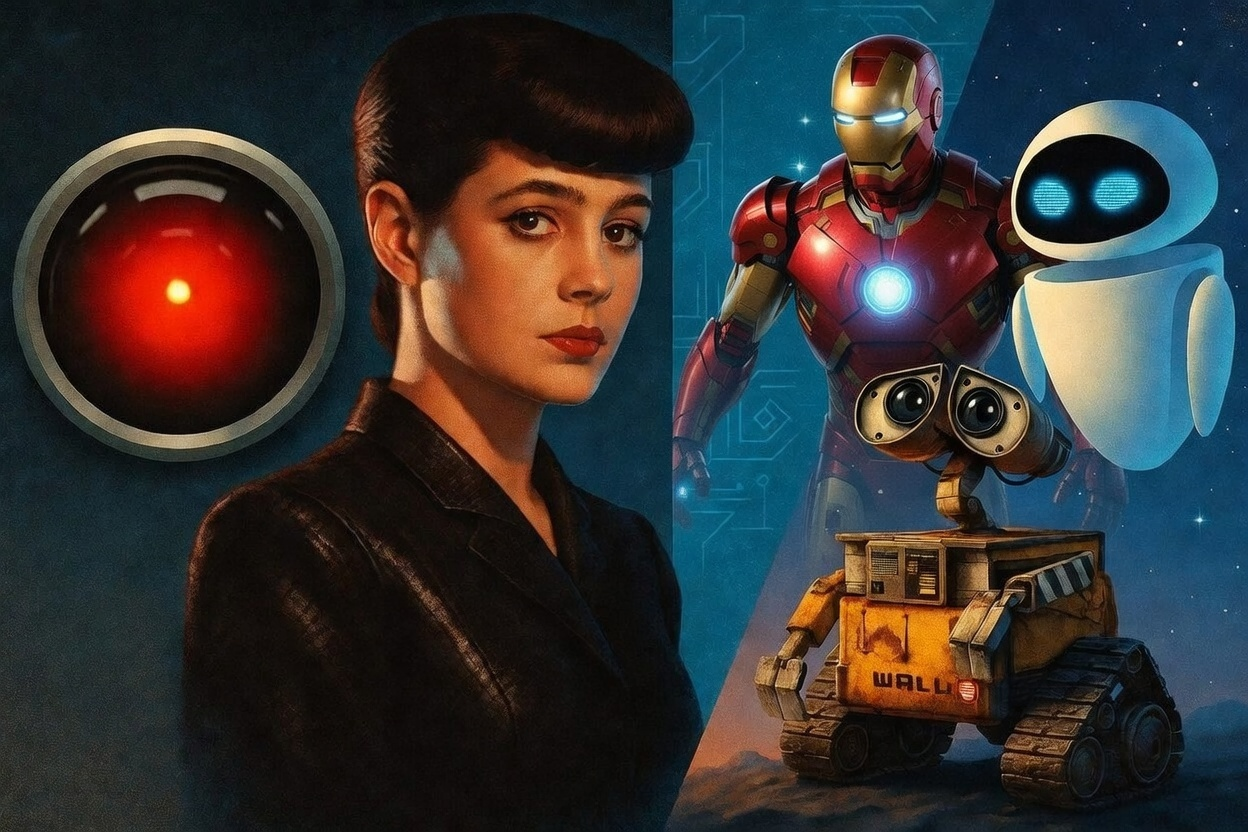
\includegraphics[width=\textwidth]{diferentesia.jpg}
            %\end{center}
        %\end{column}
    %\end{columns}
%\end{frame}

\begin{frame}{O Ecossistema da Inteligência Artificial}
    \begin{center}
        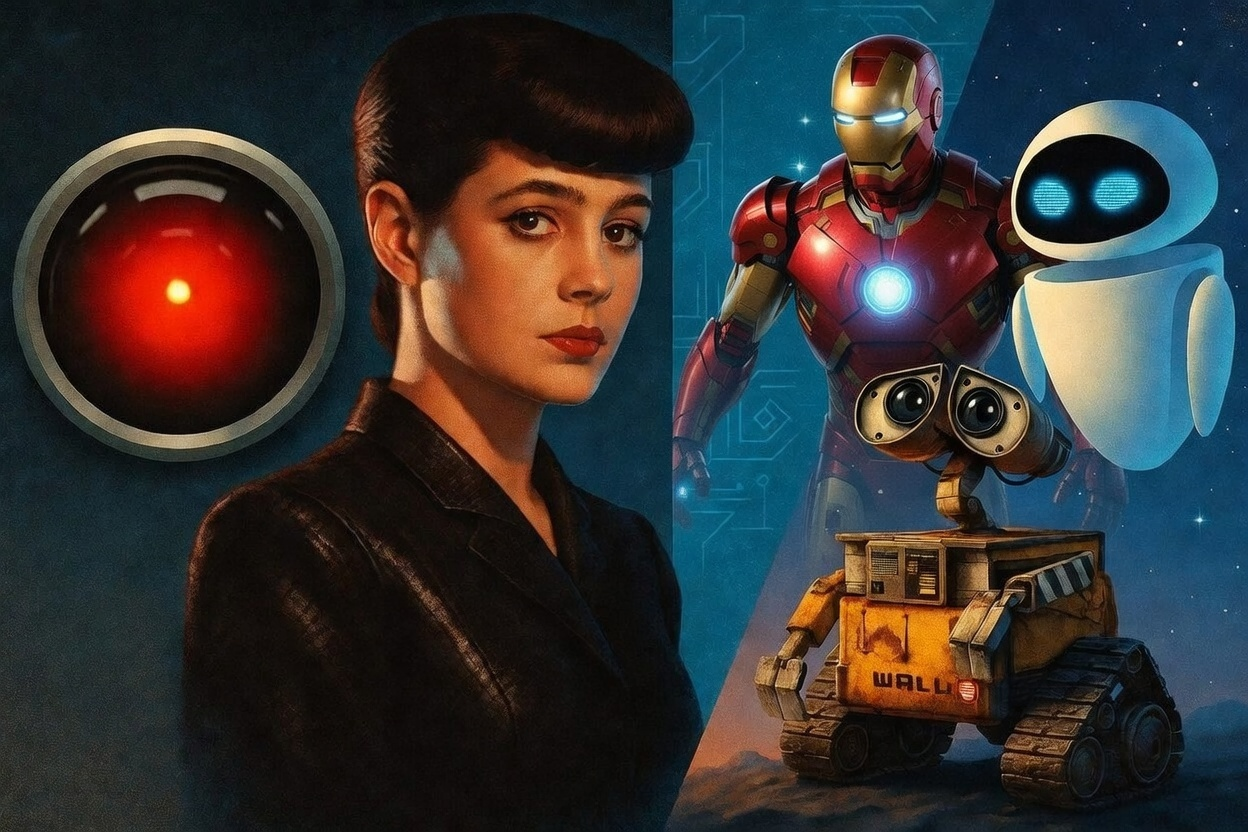
\includegraphics[scale=0.18]{diferentesia.jpg}
    \end{center}
\end{frame}

\begin{frame}{O que é Inteligência Artificial Generativa?}
    \begin{columns}
        \begin{column}{0.6\textwidth}
            \begin{block}{Diferencial Estratégico}
                Não apenas agrupa informações, mas \textbf{cria} conteúdos inéditos:
                \begin{itemize}
                    \item \faFile\, Textos, resenhas e artigos científicos
                    \item \faImage\, Imagens e simulações gráficas
                    \item \faVideo\, Vídeos e recortes audiovisuais
                    \item \faCode\, Códigos fonte (Python, C++, LaTeX)
                \end{itemize}
            \end{block}
        \end{column}
        \begin{column}{0.4\textwidth}
            \begin{alertblock}{O Salto}
                \centering
                \textcolor{warning}{\faLightbulb} \\
                \textbf{A IA saiu do plano de classificação para o plano da geração ativa!}
            \end{alertblock}
        \end{column}
    \end{columns}
\end{frame}

\begin{frame}[plain]
    \begin{center}
        \includegraphics[width=\textwidth,page=5]{apresentacao_ia_itapeva.pdf}
    \end{center}
\end{frame}

% ============================================================================
% SEÇÃO 2: SOFTWARE 3.0
% ============================================================================

\section{Software 3.0}

\begin{frame}{A Mudança de Paradigma: Software 3.0}
     \begin{columns}[T]
        \begin{column}{0.31\textwidth}
            \begin{block}{Software 1.0}
                \faCode\\
                Ações e laços lógicos programados inteiramente por desenvolvedores em linguagens duras (C, Java).
            \end{block}
        \end{column}
        \begin{column}{0.31\textwidth}
            \begin{block}{Software 2.0}
                \faSitemap\\
                Redes neurais treinadas com grandes bases de dados limitadas (reconhecimento fotográfico e padrões específicos).
            \end{block}
        \end{column}
        \begin{column}{0.31\textwidth}
            \begin{exampleblock}{Software 3.0}
                \faComments\\
                \textbf{Modelos Multimodais Massivos} controlados por linguagem natural (Inglês, Português).
            \end{exampleblock}
        \end{column}
    \end{columns}
    
    \vspace{0.5cm}
    \begin{center}
        \textbf{Hoje, o idioma global para se programar é a nossa própria fala estruturada.}
    \end{center}
\end{frame}

% ============================================================================
% SEÇÃO 3: A ABUNDÂNCIA DA INTELIGÊNCIA
% ============================================================================

\section{A Abundância da Inteligência}

\begin{frame}{O Reflexo: A Inteligência como "Commodity"}
    \begin{block}{A Reflexão Prática de Andrej Karpathy (ex-Tesla, OpenAI)}
        \textit{"Eu entendi isso intuitivamente errado por décadas, talvez por causa de uma veneração cultural pervasiva da inteligência presente na mídia, na obsessão com QI... Agência é significativamente mais poderosa e significativamente mais escassa."}
    \end{block}
    
    \begin{alertblock}{A Ruptura do Monopólio}
        \begin{itemize}
            \item Historicamente, a \textbf{Universidade} era a porta exclusiva de acesso ao conhecimento e ao exercício analítico superior (A Torre de Marfim).
            \item Hoje, sistemas na nuvem processam cálculos astrofísicos, codificam e desenham mapas moleculares em poucos segundos.
        \end{itemize}
    \end{alertblock}
\end{frame}

\begin{frame}{O Que Acontece com a Formação Tradicional?}
    \begin{itemize}
        \item Criamos, ao longo de séculos, todo um aparato institucional para medir memorização e processamento rudimentar.
        \item Cremos que o isolamento do "gênio no laboratório" seria o suficiente para transferir tecnologias milagrosas para o Brasil.
    \end{itemize}
    
    \begin{columns}
        \begin{column}{0.48\textwidth}
            \begin{alertblock}{O Passado}
                O diferencial do bom profissional: \textbf{Saber as respostas formais}.
            \end{alertblock}
        \end{column}
        \begin{column}{0.48\textwidth}
            \begin{exampleblock}{O Presente e Futuro}
                A inteligência bruta e técnica agora está \textit{"disponível na torneira"}. Qual o verdadeiro diferencial?
            \end{exampleblock}
        \end{column}
    \end{columns}
\end{frame}

\begin{frame}{O Que se Torna Escasso? A Economia Relacional}
    \begin{alertblock}{A Teoria de Alex Imas: A Pós-Commodity}
        Quando a Inteligência Artificial torna a produção de bens abstratos uma \textit{commodity} com custo marginal baixo, \textbf{o que ganha valor é aquilo que não pode ser facilmente replicado.}
    \end{alertblock}
    
    \vspace{0.3cm}
    \begin{columns}[T]
        \begin{column}{0.48\textwidth}
            \begin{block}{\faChartLine\, Elasticidade de Renda}
                À medida que a sociedade enriquece via abundância técnica, o financiamento reorienta-se para a \textbf{Economia Relacional}: setores onde o elemento humano, a exclusividade e a curadoria \textit{são parte vital do produto}.
            \end{block}
        \end{column}
        \begin{column}{0.48\textwidth}
            \begin{exampleblock}{\faHandsHelping\, O Novo Direcionador}
                A IA tira o prêmio principal do "saber escrever o relatório" técnico e o deposita no "saber olhar no olho da liderança civil" durante o processo.
            \end{exampleblock}
        \end{column}
    \end{columns}
\end{frame}

% ============================================================================
% SEÇÃO 4: O QUE É AGÊNCIA?
% ============================================================================

\section{O que é Agência?}

\begin{frame}{Agência: O Recurso Escasso Universitário}
    \begin{columns}
        \begin{column}{0.4\textwidth}
            \begin{center}
                {\Huge \textcolor{accent}{\faRunning}}
                \vspace{0.5cm}
                
                \textbf{AGÊNCIA}\\
                O princípio vivo de modular, testar e executar a inteligência.
            \end{center}
        \end{column}
        \begin{column}{0.6\textwidth}
            \begin{block}{Em Termos Práticos...}
                \begin{itemize}
                    \item A capacidade não de ler o projeto em PDF, mas de arriscar a \textbf{primeira reunião com uma prefeitura local}.
                    \item Ser proativo: não esperar o professor propor o estudo de caso, mas traze-lo da rua para a aula.
                    \item A resiliência sustentada frente à incerteza da execução (diferente da mera "hiperatividade" de mandar ideias sem fim no grupo de WhatsApp e não finalizar nenhuma).
                \end{itemize}
            \end{block}
        \end{column}
    \end{columns}
\end{frame}

\begin{frame}{Agência x Execução Guiada}
    \begin{exampleblock}{O Abismo Corporativo e do Setor Público}
        Muitos laboratórios se contentam com mestres e doutores que são excelentes "cumpridores rigorosos do que o orientador pede".
    \end{exampleblock}

    \begin{center}
        \textbf{Mas quem aponta a "seta"?} \\
        Se uma IA pode agora desenhar o cronograma técnico perfeito, quem atua socialmente para garantir que esse projeto seja implantado em uma cooperativa regional? O agente que arrisca errar!
    \end{center}
\end{frame}

% ============================================================================
% SEÇÃO 5: NOVO MODELO EDUCACIONAL
% ============================================================================

\section{Novo Modelo Educacional}

\begin{frame}{A Virada nas Premissas de Ensino}
    \begin{block}{\faSync\, Pilares para Cultivar a Agência}
        \begin{enumerate}
            \item \textbf{Privilegiar as Perguntas:} Um sistema universitário moderno deve avaliar os alunos com base também na perspicácia social dos questionamentos que eles fazem, e não mais se sabem declamar artigos já memorizados perfeitamente na LLM.
            \item \textbf{Cultura de Menos Receita, Mais Criação:} Acabar com simulações de metodologias ativas, onde o problema já é inteiramente dado e mastigado pelo docente.
            \item \textbf{Despenalizar a Falha Precoce:} Punir duramente os erros exploratórios das equipes (no modelo "Zero na Prova") funciona contra o ganho real de agência e inibe inovações. 
        \end{enumerate}
    \end{block}
\end{frame}

% ============================================================================
% SEÇÃO 6: AÇÕES DA UNESP E GOVERNANÇA (Resolução 13/2025)
% ============================================================================

\section{Ações da Unesp}

\begin{frame}{A Vanguarda da Nossa Instituição}
    \begin{exampleblock}{Ações Iniciais}
        A Unesp compreendeu que, diante da desregulação de mercado, a academia precisa ser agente regulador e fomentador ético da IA.
    \end{exampleblock}
    
    \begin{block}{A Resolução Unesp nº 13/2025}
        Estabelece políticas e diretrizes para padronizar o uso de Inteligência Artificial em nossas frentes de vanguarda: Pesquisa, Extensão, Ensino e Gestão Executiva interna da Universidade.
    \end{block}
\end{frame}

\begin{frame}{Princípios da Resolução Unesp}
    \begin{alertblock}{O Valor Maior: Ação Humana Intransferível}
        \centering
        \faUsers\, \textbf{A IA na Unesp deve atuar como força de apoio e ampliação das nossas capacidades socioeducativas, mas jamais suplantar a insubstituibilidade do tato humano.}
    \end{alertblock}
    
    \begin{columns}[T]
        \begin{column}{0.48\textwidth}
            \begin{itemize}
                \item \textbf{\faUserCheck\, Supervisão e Validação:} Decisões cruciais exigem escrutínio humano ativo.
                \item \textbf{\faBullhorn\, Transparência Autoral:} Comunicação pública se a IA co-escreveu laudos extensos ou artigos.
            \end{itemize}
        \end{column}
        \begin{column}{0.48\textwidth}
            \begin{itemize}
                \item \textbf{\faBalanceScale\, Uso Ético Responsável:} Proibir e mapear vieses discriminatórios.
                \item \textbf{\faGlobe\, Sensibilidade Socioambiental:} Conscientização da vasta pegada hídrica e carbonífera das operações em servidores de IA.
            \end{itemize}
        \end{column}
    \end{columns}
\end{frame}

\begin{frame}{Inovação Fomentada pelas Ações da Unesp}
    A universidade age legalmente não só para frear distorções, mas para \textbf{catalisar frentes mercadológicas de IA e extensão}.
    
    \begin{block}{Fomento (Resolução 13/2025 - Inovação)}
        \begin{itemize}
            \item \textbf{Parcerias Públicas e Externas:} Autorização e norte seguro para incubadoras tecnológicas, garantindo o "DNA" da Unesp em inovações colaborativas conjuntas com \textit{stakeholders} externos.
            \item \textbf{Criação de Spin-offs de Impacto:} A gestão abraça e corrobora o empreendedorismo dos campi, atrelando projetos de IA de bancada à constituição de Startups nativas.
        \end{itemize}
    \end{block}
\end{frame}

\begin{frame}{Ferramentas de IA da UNESP: Ações do LAF}
    \begin{alertblock}{Laboratório de Aplicações do Futuro (LAF)}
        Acesso centralizado às ferramentas oficiais próprias, garantindo um ambiente corporativo, fechado e ético para a comunidade acadêmica.
    \end{alertblock}
    
    \begin{columns}[T]
        \begin{column}{0.31\textwidth}
            \begin{block}{\faBalanceScale\, LegIA}
                \textbf{Assistente Jurídico} \\
                Tira-dúvidas sobre legislação interna baseado nas resoluções e normas da Unesp.
            \end{block}
        \end{column}
        \begin{column}{0.31\textwidth}
            \begin{block}{\faGraduationCap\, SapientIA}
                \textbf{Pesquisa Acadêmica} \\
                Integrado ao Repositório Institucional. Auxilia na busca de teses e dissertações.
            \end{block}
        \end{column}
        \begin{column}{0.31\textwidth}
            \begin{exampleblock}{\faRobot\, PitIA}
                \textbf{Acesso a LLMs} \\
                Ambiente seguro para ter acesso a modelos de linguagem variados e potencializar pesquisa e extensão.
            \end{exampleblock}
        \end{column}
    \end{columns}
\end{frame}

% ============================================================================
% SEÇÃO 7: REDES DE COOPERAÇÃO EXTENSIONISTAS
% ============================================================================

\section{Extensão e Agência na Prática}

\begin{frame}{A Extensão Universitária: O Epicentro Prático}
    \begin{exampleblock}{O Campo de Treino Natural}
        O robusto \textbf{sistema de Extensão da Unesp} e das redes conjuntas é, por design genético, o locus máximo do destrincamento da Agência.
    \end{exampleblock}

    \begin{itemize}
        \item \faSeedling\, Aqui, os alunos aplicam as "tarefas de alta capacidade lógica" empacotando soluções viáveis de sanidade, governança regional ou inovação social baseados na empatia humana que as IAs desconhecem.
        \item O ambiente de extensão expurga a barreira limitadora da universidade puramente retórica e avança nas trincheiras das prefeituras, do agronegócio e hospitais vitimados por carências reais.
    \end{itemize}
\end{frame}

\begin{frame}{A Equação Operacional do Nosso Futuro}
    \begin{center}
        \textbf{\Huge IA Analítica + Agência no Território}
    \end{center}
    
    \vspace{0.5cm}
    \begin{columns}
        \begin{column}{0.48\textwidth}
            \begin{block}{\faRobot\, O que a Máquina faz}
                Sintetiza dezenas de regulações normativas rurais em minutos, revisa documentações do projeto, cria apresentações prévias e gera modelos logísticos.
            \end{block}
        \end{column}
        
        \begin{column}{0.48\textwidth}
            \begin{block}{\faCommentDots\, O que a Rede Extensionista faz}
                Realiza o acordo na Câmara Municipal com as representações civis, cria a interlocução de confianças interpessoais vitais e encampa o convencimento orgânico para o uso das ferramentas.
            \end{block}
        \end{column}
    \end{columns}
\end{frame}

% ============================================================================
% ENCERRAMENTO
% ============================================================================

\section{Encerramento}

\begin{frame}{Desafio Estratégico (O Balanço Final)}
    \begin{alertblock}{As Perguntas Reflexivas para o nosso Sistema}
        \begin{enumerate}
            \item Nós, na condição de orientadores e líderes de setor, estamos valorizando a Agência Extensionista como critério definitivo da formação?
            \item Você está agindo em sala de aula como se a "inteligência crua" fosse ainda um fator determinante nos próximos 5 anos?
            \item Nossa ação extensionista no contexto brasileiro é proativa (moduladora) ou reativa?
        \end{enumerate}
    \end{alertblock}
\end{frame}

\begin{frame}
    \begin{center}
        {\Huge \textcolor{accent}{Muito Obrigado!}}
        
        \vspace{1cm}
        \faEnvelope\, ney.lemke@unesp.br \\
        \faGlobe\, www.unesp.br/ctinf 
        
        \vspace{1cm}
        \textit{"Se o poder de computação do planeta está à distância de um prompt de teclado... a Agência para moldar a nossa realidade local com empatia, segue sendo um recurso valioso e irreplicável."}
    \end{center}
\end{frame}

\end{document}
